\section{Results}
\subsection{Results of the datasets}
The results of the MATLAB code calculating $k_{trap,x}$ and $k_{trap,y}$ for the two data sets are presented in table \ref{tab:first-results}. Since the MATLAB code failed to track the bead for some of the measurements in the first data set, not all values are used for fitting. The second dataset was much better and did not have any faulty measurements. The corresponding values are shown in table \ref{tab:second-results}.\\

\vspace{-.2cm}
\begin{table}[h!]
\centering
\begin{tabular}{|l|l|l|l|l|l|l|}
\hline
Laser Power {[}$mW${]} & 0*         & 10*        & 20        & 30*        & 40         & 40        \\ \hline
$k_{trap,x}$    {[}$pN/nm${]}        & $2.36 \cdot 10^{-5}$ &$ 2.45 \cdot 10^{-7}$ & $1.60\cdot 10^{-5}$  & $8.35\cdot 10^{-7}$ & $1.99\cdot 10^{-5}$  & $9.60\cdot 10^{-5}$ \\ \hline
$k_{trap,y}$     {[}$pN/nm${]}       & $8.29 \cdot 10^{-5}$ &$ 2.94\cdot 10^{-7}$ & $1.65\cdot 10^{-5}$ & $9.71\cdot 10^{-7}$ & $1.72\cdot 10^{-5}$ & $8.96\cdot 10^{-5}$ \\ \hline
\end{tabular}
\caption{Results of the first dataset. The values are truncated to two decimal places. * denotes a faulty measurement}
\label{tab:first-results}
\end{table}


\vspace{-.2cm}
\begin{table}[h!]
\centering
    \begin{tabular}{|l|l|l|l|l|l|l|}
        \hline
        Laser Power {[}$mW${]} & 0         & 5         & 10         & 20         & 30         & 40         \\ \hline
        $k_x$     {[}$pN/nm${]}       & $3.64\cdot 10^{-7}$ & $8.24\cdot 10^{-5}$ & $1.08\cdot 10^{-4}$ & $3.03\cdot 10^{-4}$ & $6.14\cdot 10^{-4}$ & $7.55\cdot 10^{-4}$ \\ \hline
        $k_y$     {[}$pN/nm${]}       & $5.55\cdot 10^{-7}$   & $4.18\cdot 10^{-5}$ & $2.53\cdot 10^{-5}$  & $1.10\cdot 10^{-4}$ & $1.69\cdot 10^{-4}$ & $2.54\cdot 10^{-4}$ \\ \hline
    \end{tabular}
\caption{Trap results, values are truncated to two decimal places for formatting reasons}
\label{tab:second-results}
\end{table}

We cannot calculate the exact value of the error since the MATLAB algorithm does not provide us with the locations and its error. However, if we estimate the error of the bead location to be $u_{xi} = l_{pixel}/2$ and we know that 1000 frames were used for the calculation of the trap constants we find from equation \ref{eq_u_k_constant} that $u_{k_{trap}} = l_{pixel} (k_B T)^{\frac{1}{2}}  k_{trap} ^{\frac{3}{2}}$. However when these values are calculated we see an error between $0.1\%$ and $0.00001\%$ of that of the $k_{i}$ value, these values are lower then we believe they should be. We suspect that this is the case since the MATLAB algorithm confidently tracks a incorrect stationary artefact on the trap surface.


\begin{minipage}{\linewidth}[h!]
    \begin{minipage}[l]{0.45\linewidth}
        \begin{figure}[H]
            \centering
            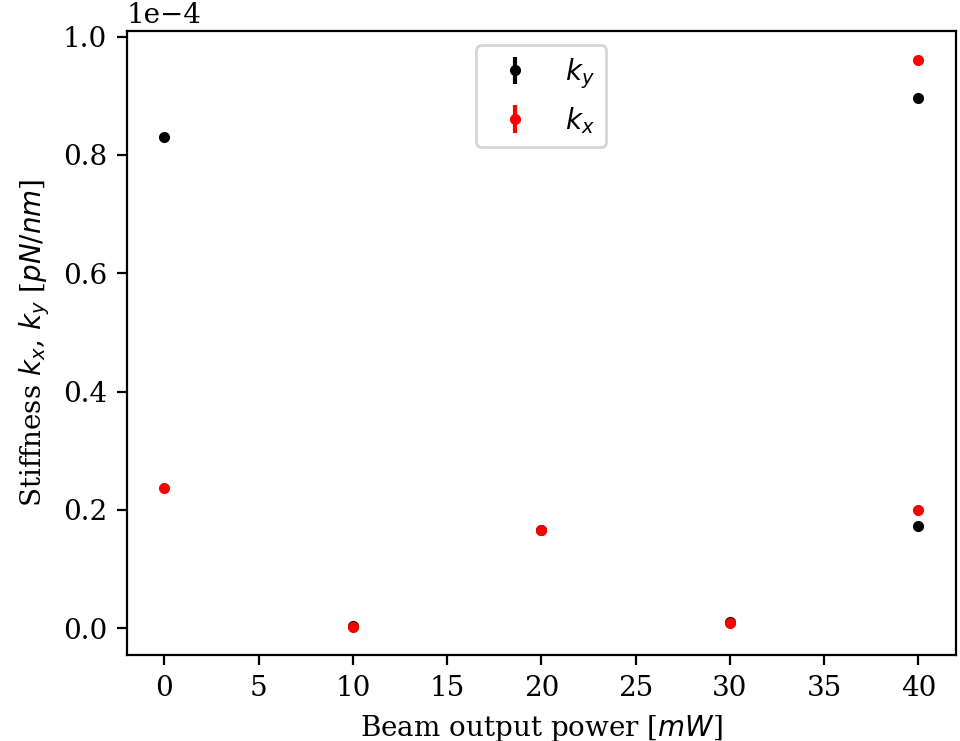
\includegraphics[width=\linewidth]{figures/beam.png}
            \caption{Results of the first dataset plotted and fitted.\\}
            \label{fig:bead-plot}
        \end{figure}
    \end{minipage}
    \hfill
    \begin{minipage}[r]{0.45\linewidth}
        \begin{figure}[H]
            \centering
            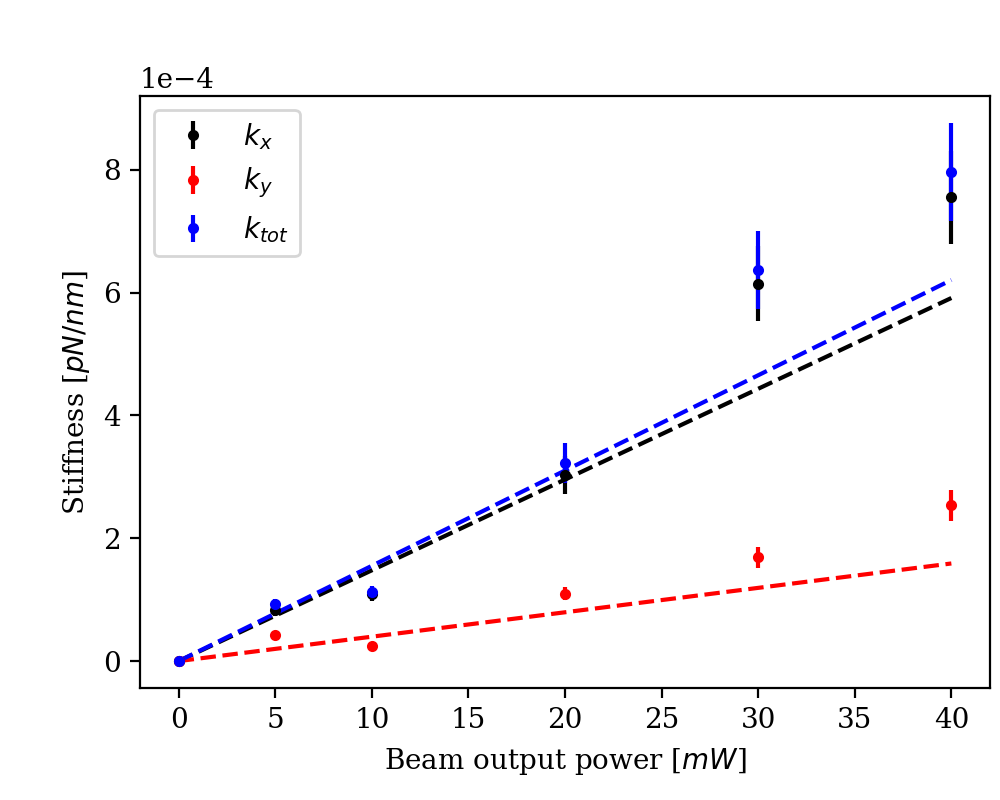
\includegraphics[width=\linewidth]{figures/trap.png}
            \caption{Results of the second dataset plotted and fitted.\\}
            \label{fig:trap-plot}
        \end{figure}
    \end{minipage}

\end{minipage}
\\

The data shown above in tables \ref{tab:first-results} and \ref{tab:second-results} are plotted in figures \ref{fig:bead-plot} and \ref{fig:trap-plot} re\-spectively. In the plots the in\-divi\-dual data points are plotted. For the first dataset no reasonable fit could be made corresponding with the expected linear relation. For the second dataset, a least squares fit for $k_x$ and $k_y$ to the linear relation to the laser power is plotted.

The corresponding values for the correlation constants are $ \alpha_x = 1.5 \; \pm 0.5 \; \cdot 10^{-5}$ and $\alpha_y = 4 \; \pm 1 \; \cdot 10^{-6}$

\begin{comment}

The resulting values of $\alpha$ for the least squares fit to the function $k_{trap}= \alpha \cdot P$  are shown below in table \ref{tab:fit-results}.

\vspace{-0.5cm}
\begin{table}[h!]
    \centering
    \begin{tabular}{|l|l|l|}
        \hline
        coefficient for & $\alpha_x$ {[}$pN/(nm\cdot mW)${]} & $\alpha_y$ {[}$pN/(nm \cdot mW)${]}\\ \hline
        dataset 1       & $1.382\cdot 10^{-6}$          & $1.280 \cdot 10^{-6}$\\ \hline
        dataset 2       & $1.478 \cdot 10^{-5}$         & $3.974 \cdot 10^{-6}$\\ \hline
    \end{tabular}
    \caption{The results of the linear fits for the trap stiffness as a function of laser output power.}
    \label{tab:fit-results}
\end{table}

\end{comment}

\clearpage{}
\subsection{Python program results}
\label{results}
During this practical we were also tasked with rewriting a MATLAB script in to Python. The piece of script we needed to rewrite was the function that tracks the centre of the bead in the image, this function was comprised of interpolation method and a method that found the symmetry centre of the bead using Fourier transforms. The second part was easily implemented in Python as it was mostly just finding the right Python functions that were equivalent to their MATLAB counterparts. The interpolation function was a lot harder to implement in Python since most of the existing Python interpolation functions did not have the same functionality. The documentation of this part of the practical can be found in the appendix\\

As outlined in the section \ref{trap_constant} a method for deriving the trap constants was proposed that differs from the one from the MATLAB script. This method was implemented in a second different python script to try and show its usefulness. This python script can be found in the appendix.\\

The result speaks for itself, it shows a clear connection between the laser output power and the length of the semi-major and semi-minor axis of the ellipses that encircle the points describing the symmetry centres of the beads. The points were fitted with a function with shape $L_{axis}=\frac{\beta}{P}+\gamma$, this seems to fit well as can be seen in figure \ref{fig:spread-bead-plot} \& \ref{fig:spread-trap-plot}. This suggests that the theoretical inverse proportionality between the $\langle x^2 \rangle$ and the laser power is correct. The data corresponding to these plots are shown in table \ref{tab:axis-results-one} and in table \ref{tab:axis-results-two}. In the appendix three more plots showing the spread of the centres of mass can be seen.

\begin{minipage}{\linewidth}
    \centering
    \begin{minipage}[l]{0.45\linewidth}
        \begin{figure}[H]
            \centering
            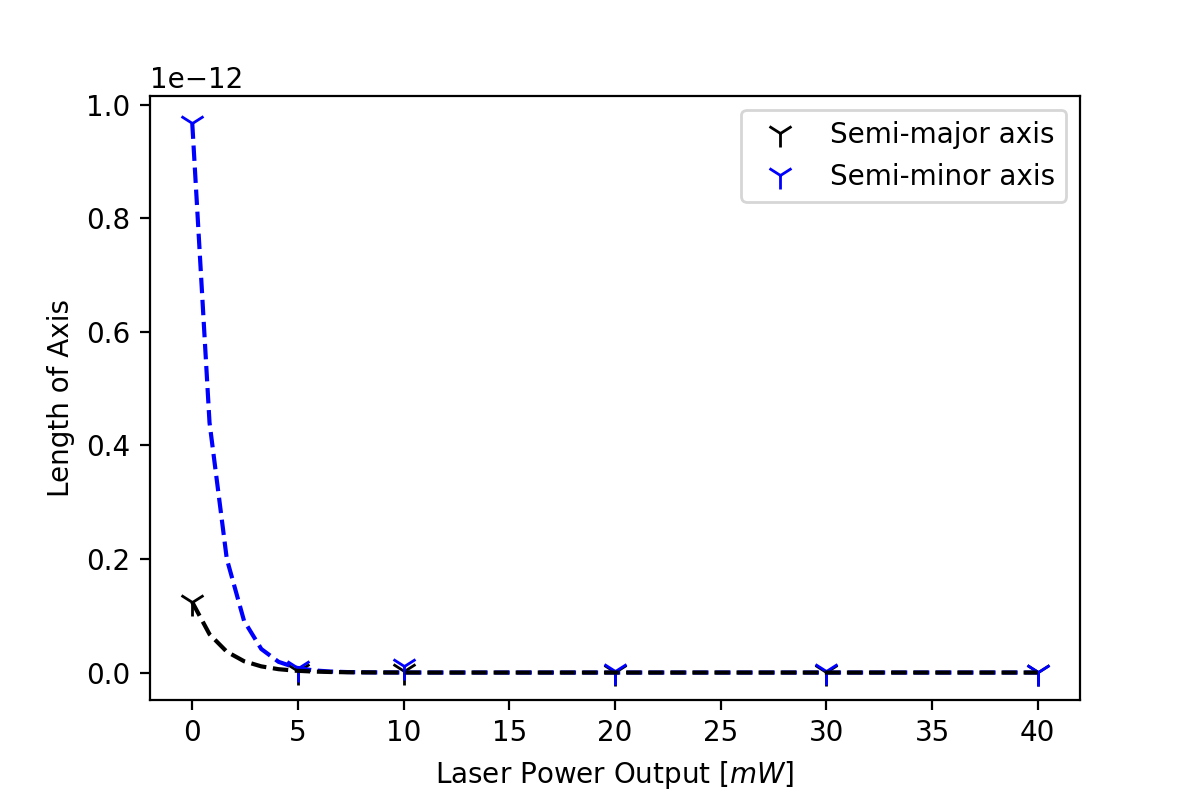
\includegraphics[width=\linewidth]{figures/axis-dataset2.png}
            \caption{Semi-major and minor axis of the first dataset plotted and fitted.\\}
            \label{fig:spread-bead-plot}
        \end{figure}
    \end{minipage}
    \hspace{0.05\linewidth}
    \begin{minipage}[r]{0.45\linewidth}
        \begin{figure}[H]
            \centering
            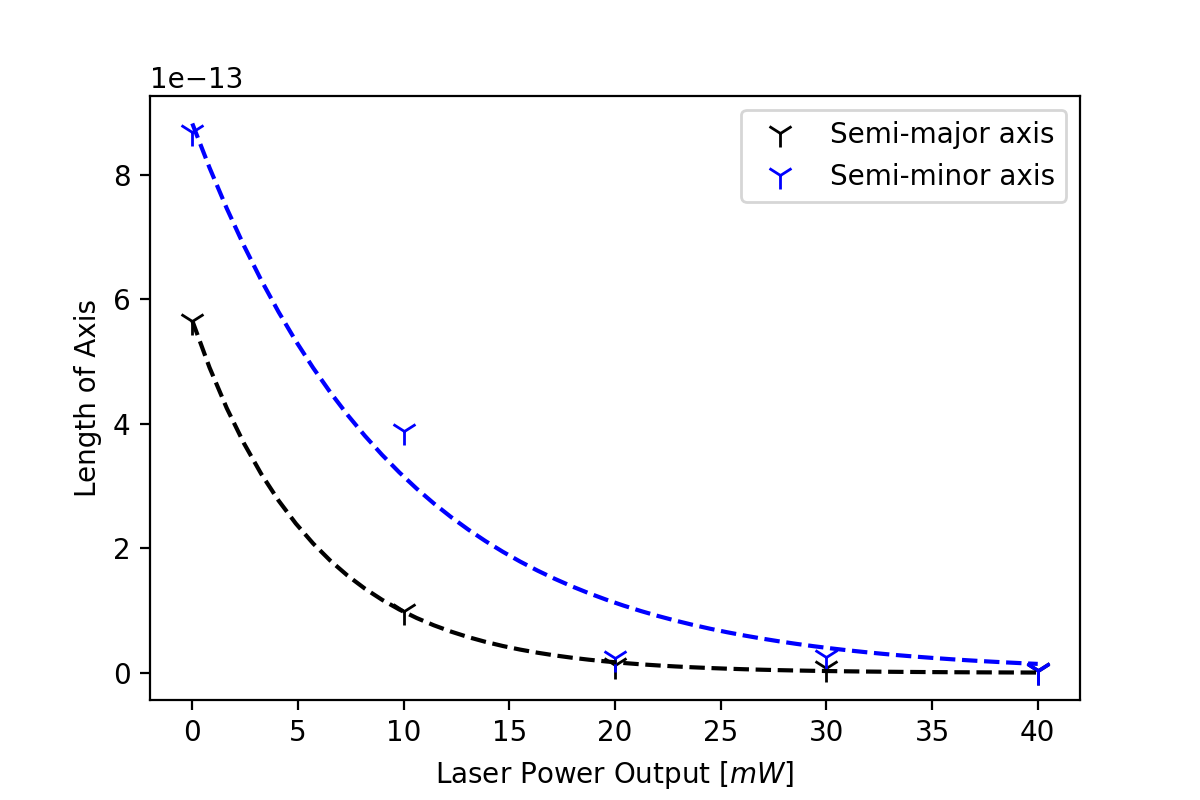
\includegraphics[width=\linewidth]{figures/axis-dataset1.png}
            \caption{Semi-major and minor axis of the second dataset plotted and fitted.\\}
            \label{fig:spread-trap-plot}
        \end{figure}
    \end{minipage}

\end{minipage}

The values for semi-major- and semi-minor-axes were acquired using the Trackpy python function. Given the values and the accuracy of the fitted lines indicates that the Trackpy function performs well for particle tracking. The difference between figure \ref{fig:bead-plot}, not showing any correlation, and figure \ref{fig:spread-bead-plot}, showing the theoretical correlation, can be explained by better performance of the Trackpy function compared to the MATLAB script for the first dataset.

\begin{table}[]
\caption{Resulting Axis lengths of dataset 1}
\label{tab:axis-results-one}
\begin{tabular}{|l|l|l|l|l|l|l|}
\hline
\multicolumn{7}{|l|}{Dataset 1}                                                                                         \\ \hline
Laser power output [$mW$] & 0                                                    & 10   & 20   & 30   & 40   & 40   \\ \hline
Semi-major-axes [$nm$]   & $8.69 \cdot 10^{-4}$ & $3.88\cdot 10^{-4}$ & $2.41\cdot 10^{-5}$ & $2.50\cdot 10^{-5}$ & $3.36\cdot 10^{-6}$ & $4.73\cdot 10^{-6}$ \\ \hline
Semi-minor-axis [$nm$]   & $5.66 \cdot 10^{-5}$ & $9.94\cdot 10^{-5}$ & $1.19\cdot 10^{-5}$ & $7.16\cdot 10^{-6}$ & $2.93\cdot 10^{-6}$ & $3.97\cdot 10^{-6}$ \\ \hline
\end{tabular}
\end{table}


\begin{table}[]
\caption{Resulting Axis lengths of dataset 1}
\label{tab:axis-results-two}
\begin{tabular}{|l|l|l|l|l|l|l|}
    \hline
    \multicolumn{7}{|l|}{Dataset 2}                                                                                         \\ \hline
    Laser power output [$mW$] & 0 &5 & 10   & 20   & 30   & 40\\ \hline
    Semi-major-axes [$nm$]   & $9.67 \cdot 10^{-4}$ & $1.22\cdot 10^{-5}$ & $3.02\cdot 10^{-6}$ & $1.86\cdot 10^{-6}$ & $1.32\cdot 10^{-6}$ & $4.73\cdot 10^{-6}$ \\ \hline
    Semi-minor-axis [$nm$]   & $1.24 \cdot 10^{-5}$ & $1.90\cdot 10^{-6}$ & $4.48\cdot 10^{-7}$ & $2.71\cdot 10^{-7}$ & $1.45\cdot 10^{-7}$ & $2.89\cdot 10^{-6}$ \\ \hline
\end{tabular}
\end{table}
